% !TEX encoding = UTF-8 Unicode

\documentclass[letterpaper,11pt]{article}

%A Few Useful Packages
%\usepackage{marvosym}
\usepackage{fontspec}     %for loading fonts
\usepackage{xunicode,xltxtra,url,parskip} 	%other packages for formatting
\usepackage{graphicx}
\usepackage[usenames,dvipsnames]{xcolor}
\usepackage[left=1.3cm,
            top=0.9cm,
            right=1.3cm,
            bottom=1.2cm,
            nohead,
            nofoot
            ]{geometry}
\usepackage{tabularx}
\usepackage{titlesec}
%\usepackage{tabto}        % tab spacing

\usepackage{setspace}     % line spacing
\usepackage{booktabs,colortbl}       % thicker rules between table cells
\usepackage{bibentry}     % bibliography

% SORTED LISTS
\usepackage{paralist}
\usepackage{datatool}% http://ctan.org/pkg/datatool
\newcommand{\sortitem}[1]{%
  \DTLnewrow{list}% Create a new entry
  \DTLnewdbentry{list}{description}{#1}% Add entry as description
}
\newenvironment{sortedlist}{%
  \DTLifdbexists{list}{\DTLcleardb{list}}{\DTLnewdb{list}}% Create new/discard old list
}{%
  \DTLsort{description}{list}% Sort list
  \begin{inparaitem}[]%
    \DTLforeach*{list}{\theDesc=description}{%
      \item \theDesc, }% Print each item
  \end{inparaitem}%
}

%Setup hyperref package, and colours for links
\usepackage[colorlinks,
            breaklinks,
            pagebackref=false,
            debug=true,
            xetex,
            bookmarks=false,
            pdfpagelabels=false,
            hyperfootnotes=false,
            hyperindex=false,
            pageanchor=false]{hyperref}
\definecolor{linkcolor}{gray}{0.2}
\hypersetup{
  pdfauthor={Amin Kasrou Aouam},
  pdfsubject={Amin Kasrou Aouam - Resume},
  pdftitle={Amin Kasrou Aouam - Resume},
  urlcolor=linkcolor,
  linkcolor=linkcolor
}
% colors
\definecolor{dark-gray}{gray}{0.15}
\definecolor{light-gray}{gray}{0.55}

%FONTS
\setmainfont{Liberation Serif}
\newfontfamily{\hlight}{Liberation Serif}
\defaultfontfeatures{Mapping=tex-text} % converts LaTeX specials (``quotes'' --- dashes etc.) to unicode
\usepackage{fontawesome5}  % glyphs for contact info

% CUSTOM COMMANDS
  \newcommand{\titlerulethick}{{%
    {\color{dark-gray} \titlerule[0.5mm] }%
  }}

  % old section title format
  \titleformat{\section}{\fontsize{28pt}{38pt}\color{dark-gray}\normalfont}{}{0mm}{}[\titlerulethick]
  %\titlespacing{\section}{0pt}{3pt}{3pt}

  \newcommand{\namefont}[1]{{%
    \fontsize{42pt}{50pt}\normalfont\textbf{#1}%
  }}

  \newcommand{\spacerule}{
    \addlinespace[0.5em]
    \midrule[0.5mm]
    \addlinespace[0.5em]
  }

  \newcommand{\bigfont}[1]{{%
    \fontsize{32pt}{38pt}\normalfont{#1} %
  }}

  \newcommand{\lightfont}[1]{{%
    {\hlight#1}
  }}

  \newcommand{\contactinfo}{%
    {\hlight\color{dark-gray}}
  }

  \newcommand{\lightsmall}[1]{{%
    {\fontsize{11pt}{14pt}\hlight#1}
  }}

  \newcommand{\pubstyle}[1]{{%
    {\fontsize{10pt}{13pt}\hlight#1}
  }}

  \newcommand{\lightbf}[1]{{%
    \textbf{\lightfont{#1}}
  }}

  \newcommand{\emphasized}[1]{{%
    {\fontsize{12pt}{14pt}\textbf{#1}}
  }}

  \newcommand{\position}[1]{{%
    {\fontsize{12pt}{14pt} \hlight{#1}}
  }}

  \newcommand{\company}[1]{{%
    {\fontsize{12pt}{14pt} \textbf{#1}}
  }}

  \newcommand{\headline}{
    {\fontsize{14pt}{17pt}\bfseries\color{dark-gray}}
  }

  \newcommand{\name}{
    \raggedright\fontsize{38pt}{38pt}\bfseries\flushleft\color{dark-gray}{Amin
Kasrou Aouam}
  }

  \newcommand{\lighthrule}{
    {\color{light-gray}\par\rule[0mm]{\hsize}{0.5mm}\par\vspace{0.0em}}
  }

% hack to remove bibliography numbering
\makeatletter
\renewcommand\@biblabel[1]{}
\renewenvironment{thebibliography}[1]
     {\section*{\refname}%
      \@mkboth{\MakeUppercase\refname}{\MakeUppercase\refname}%
      \list{}%
           {\leftmargin0pt
             \@openbib@code
             \usecounter{enumiv}}%
      \sloppy
      \clubpenalty4000
      \@clubpenalty \clubpenalty
      \widowpenalty4000%
      \sfcode`\.\@m}
     {\def\@noitemerr
       {\@latex@warning{Empty `thebibliography' environment}}%
      \endlist}
\makeatother
%
%-------------------- BEGIN DOCUMENT ----------------------
\begin{document}
%\nocite{}
\pagestyle{empty} % non-numbered pages
\font\fb=''[cmr10]'' %for use with \LaTeX command
%---------- SPECIFY LENGTHS ----------
\newlength{\leftwide}
\setlength{\leftwide}{0.34\textwidth}
%
\newlength{\centerwide}
\setlength{\centerwide}{0.33\textwidth}
%
\newlength{\rightwide}
\setlength{\rightwide}{0.28\textwidth}
%---------- TOP SECTION ----------
\begin{tabular}[b]{@{}p{\leftwide}@{}p{\centerwide}@{}p{\rightwide}@{}}
  % NAME (left)
  \noindent
  \begin{minipage}[b]{\leftwide}
    \name
  \end{minipage} & %
  % CONTACT INFO (middle)
  \begin{minipage}[b]{\centerwide}
    \renewcommand\arraystretch{1.25}
    \contactinfo
    \begin{tabular}[b]{@{}cl@{}}
      \faEnvelope & \href{mailto:akasroua@gmail.com}{akasroua@gmail.com}\\ %{}
      \faPhone & +34 658591161\\
      \faGitlab & \href{https://gitlab.com/akasroua}{gitlab.com/akasroua}\\
    \end{tabular}
  \end{minipage} & %
% PHOTO (right)
  \begin{minipage}[b]{\rightwide}
    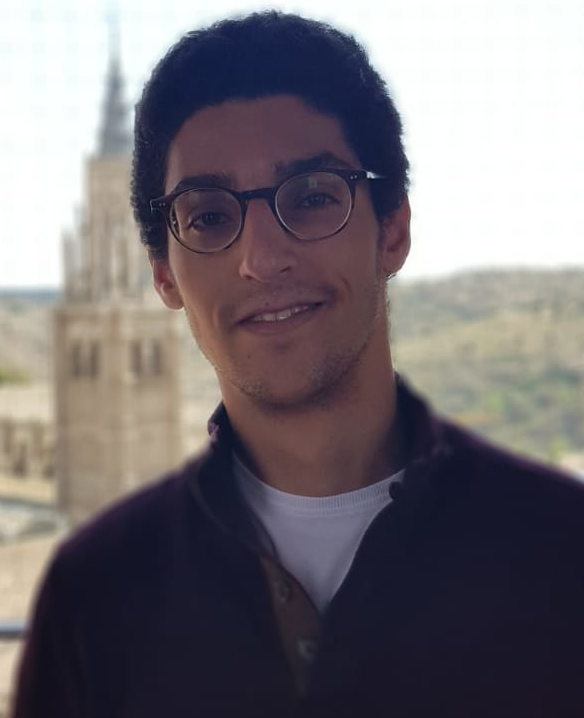
\includegraphics[width=7em]{Assets/photo.png}
  \end{minipage} 
\end{tabular}
%---------- MAIN BODY ----------
% ABOUT
\vspace{-3.2em}
{\section{}
\parbox[t][][t]{\textwidth}{
    Estudiante de Ingeniería Informática, interesado en las áreas de
    inteligencia artificial, bioinformática, infraestructura como código
    (IaC), sistemas distribuidos e inmutables.

    Busco una oportunidad laboral instructiva, con un énfasis en el
    trabajo en grupo y la colaboración.
}
%---------- LEFT SIDE ----------
\newlength{\hwide}
\begin{minipage}[t]{0.31\textwidth}
  \raggedright
    % PROGRAMMING
    \ifthenelse{\equal{es}{en}}
        {\section{programming}}
        {\section{programación}}%
    \setlength{\parskip}{1mm}
    \setlength{\hwide}{\dimexpr.5\hsize-3\tabcolsep}
    %
    \hlight
    \begin{tabular}{@{}p{\hwide}p{\centerwide}}
              \parbox[t][][t]{\hwide}{%
          \emphasized{Python}
          \medskip
        } & %
        \parbox[t][][t]{\centerwide}{%
          \lightbf{Avanzado}
          \medskip
        } \\ %
              \parbox[t][][t]{\hwide}{%
          \emphasized{C++}
          \medskip
        } & %
        \parbox[t][][t]{\centerwide}{%
          \lightbf{Intermedio}
          \medskip
        } \\ %
              \parbox[t][][t]{\hwide}{%
          \emphasized{Nix}
          \medskip
        } & %
        \parbox[t][][t]{\centerwide}{%
          \lightbf{Intermedio}
          \medskip
        } \\ %
              \parbox[t][][t]{\hwide}{%
          \emphasized{Java}
          \medskip
        } & %
        \parbox[t][][t]{\centerwide}{%
          \lightbf{Básico}
          \medskip
        } \\ %
              \parbox[t][][t]{\hwide}{%
          \emphasized{PHP}
          \medskip
        } & %
        \parbox[t][][t]{\centerwide}{%
          \lightbf{Básico}
          \medskip
        } \\ %
          \end{tabular}

    % TECHNOLOGIES
    %
    \ifthenelse{\equal{es}{en}}
        {\section{technical skills}}
        {\section{tecnologías}}%
    \hlight
    \begin{itemize}[]
            \item{Linux/FreeBSD}
            \item{\LaTeX}
            \item{Git}
            \item{LEMP Stack}
            \item{APIs REST}
            \item{SQL}
            \item{NixOS}
          \end{itemize}

    % COURSES
    %
    \ifthenelse{\equal{es}{en}}
        {\section{courses}}
        {\section{cursos}}%
    \hlight
        \emphasized{Fundamentos de Robótica} \\
    \lightfont{\textbf{Adams Formación}} \\
        \emphasized{Programación con Python} \\
    \lightfont{\textbf{Universidad de Granada}} \\
        \emphasized{Programación y distribución de aplicaciones móviles
para dispositivos Android e IOS} \\
    \lightfont{\textbf{Universidad de Granada}} \\
        \emphasized{Arduino} \\
    \lightfont{\textbf{Universidad de Granada}} \\
    \end{minipage}%
%
%---------- RIGHT SIDE ----------
\newlength{\hwideright}
\newlength{\buffer}
\setlength{\buffer}{4pt plus 1pt minus 1pt}
%
\begin{minipage}[t]{0.64\textwidth}
  % EXPERIENCE
  \ifthenelse{\equal{es}{en}}
      {\section{experience}}
      {\section{experiencia laboral}}%
  \setlength{\hwide}{\dimexpr.5\hsize-4\tabcolsep}
  \setlength{\hwideright}{\dimexpr\hwide+5\tabcolsep}
  %
  \begin{tabular}{@{}p{\hwide}p{\hwideright}}
    \arrayrulecolor{light-gray}
          \parbox[t][][t]{\hwide}{%
          \raggedright
          \company{JITKey}\\
          \vspace{\buffer}
          \lightfont{%
          Febrero 2020 \textendash{} Marzo 2020\\
                    \vspace{\buffer}}
                  } & %
      \parbox[t][][t]{\hwideright}{%
          \raggedright
          \position{Prácticas}\\
          \vspace{\buffer}
          \lightsmall{Responsable de Soporte en una startup española.
Suspendidas debido al COVID-19}
        }\\
      \end{tabular}
  % EDUCATION
  \ifthenelse{\equal{es}{en}}
      {\section{education}}
      {\section{formación académica}}%
  \setlength{\hwide}{\dimexpr.5\hsize-4\tabcolsep}
  \setlength{\hwideright}{\dimexpr\hwide+5\tabcolsep}
  % 
  \setlength{\parskip}{1mm}
  \vspace{-0.5em}
  \begin{tabular}{@{}p{\hwide}p{\rightwide}}
          \parbox[t][][t]{\hwide}{%
        \lightfont{2017 \textendash{} presente} \\
        \smallskip
        \emphasized{Grado} \\
        \smallskip
        \emphasized{Ingeniería Informática} \\
      } & %
      \parbox[t][][t]{\rightwide}{%
        \lightfont{\textbf{Universidad de Granada} \\
          \emph{Ceuta}} \\ %
        \medskip %
      } \\
          \parbox[t][][t]{\hwide}{%
        \lightfont{2015 \textendash{} 2017} \\
        \smallskip
        \emphasized{Grado} \\
        \smallskip
        \emphasized{Medicina} \\
      } & %
      \parbox[t][][t]{\rightwide}{%
        \lightfont{\textbf{Universidad de Sevilla} \\
          \emph{Sevilla}} \\ %
        \medskip %
      } \\
          \parbox[t][][t]{\hwide}{%
        \lightfont{2013 \textendash{} 2015} \\
        \smallskip
        \emphasized{Grado} \\
        \smallskip
        \emphasized{Medicina} \\
      } & %
      \parbox[t][][t]{\rightwide}{%
        \lightfont{\textbf{Université Paris-Sud} \\
          \emph{Châtenay-Malabry}} \\ %
        \medskip %
      } \\
      \end{tabular}
  \vspace{-0.8em}
  % 

  % LANGUAGES
  \ifthenelse{\equal{es}{en}}
      {\section{languages}}
      {\section{idiomas}}%
  %
  \setlength{\parskip}{1mm}
  \setlength{\hwide}{\dimexpr.5\hsize-4\tabcolsep}
  \setlength{\hwideright}{\dimexpr\hwide+5\tabcolsep}

  \begin{tabular}{@{}p{\hwide}p{\rightwide}}
          \parbox[t][][t]{\hwide}{%
        \emphasized{Inglés}
        \medskip
      } & %
      \parbox[t][][t]{\rightwide}{%
        \lightbf{Fluido}
        \medskip
      } \\ %
          \parbox[t][][t]{\hwide}{%
        \emphasized{Español}
        \medskip
      } & %
      \parbox[t][][t]{\rightwide}{%
        \lightbf{Nativo}
        \medskip
      } \\ %
          \parbox[t][][t]{\hwide}{%
        \emphasized{Francés}
        \medskip
      } & %
      \parbox[t][][t]{\rightwide}{%
        \lightbf{Nativo}
        \medskip
      } \\ %
          \parbox[t][][t]{\hwide}{%
        \emphasized{Darija (Dialecto marroquí)}
        \medskip
      } & %
      \parbox[t][][t]{\rightwide}{%
        \lightbf{Nativo}
        \medskip
      } \\ %
      \end{tabular}
%
%\section{publications}
%\vspace{-0.5em}
%\begingroup
%\renewcommand{\section}[2]{}%
%\pubstyle{
%  \bibliography{pubs}
%  \bibliographystyle{cvbib}
%}
%\endgroup
\end{minipage}
% ==========================================================
%-------------------- END OF DOCUMENT ----------------------
\end{document}
